\documentclass[a4paper]{llncs}
\usepackage{url}
\usepackage{graphicx}
\usepackage{multirow}
\usepackage{comment}
\usepackage{subfigure}
\usepackage{printlen} % Print lengths using specified units. 
%\usepackage{hyperref}
\usepackage{booktabs}
\usepackage[utf8]{inputenc} % Umlaute üöä auch normal benutzen und nicht maskieren
\usepackage[rightcaption]{sidecap}  % caption beside figure
\usepackage{color}
\usepackage{amsmath, amssymb, array}
\usepackage{listings}
\usepackage{subfigure}
\usepackage{color}
\usepackage{todonotes}
\usepackage{enumerate}
\usepackage{array}
\usepackage{spverbatim}

% http://www.ctan.org/tex-archive/fonts/ps-type1/cm-super/
\usepackage[T1]{fontenc} % use high quality fonts, please install cm-super


%%%% LISTINGS
\usepackage{listings} % Typeset source code listings using LaTeX.
% listing styles
\lstset{
    numberbychapter=false,
    numbers=left,
    numberstyle=\tiny,
    basicstyle=\ttfamily\fontsize{8}{8}\selectfont,
    tabsize=2,
    framexleftmargin=2pt,
    captionpos=b,
    frame=single,
    breaklines=true
}

% Turtle box
\usepackage{color}
\definecolor{olivegreen}{rgb}{0.1,0.6,0.3}
\definecolor{grey}{rgb}{0.2,0.2,0.2}
\lstdefinelanguage{ttl}{
sensitive=true,
showstringspaces=false,
morecomment=[l][\color{grey}]{@},
morecomment=[l][\color{olivegreen}]{\#},
morestring=[b][\color{blue}]\",
keywordstyle=\color{cyan},
morekeywords={version,owl,rdf,rdfs,xml,xsd,dbo,str,sso,scms,ld, fise, dcterms, itsrdf, wiktionary, nif, rlno, dbpedia,rlnr}
}

%\lstdefinestyle{rdf}{numberblanklines=true, morekeywords={}}
%\lstdefinestyle{sparql}{numberblanklines=true, morekeywords={SELECT,WHERE FILTER, GROUP BY, IN, AS}}
\lstdefinestyle{N3}{numberblanklines=true, morekeywords={foaf, prefix}}

%%%% todo
% \newcommand{\todo}[1]{\textbf{[ToDo: #1]}}
% draws PDF notes instead of in-text todos
%\usepackage{pdfmarginpar}\newcommand{\todo}[1]{\pdfmarginpar[Note]{ToDo: #1}}
%\newcommand{\todo}[1]{}

\pdfinfo{                                                                               
	/Title (Real-time RDF extraction from unstructured data streams)
	/Creator (TeX)                                                                      	
	/Producer (pdfTeX and Document $Revision: 5900 $)
	/Author (Daniel Gerber, Lorenz Bühmann, Tommaso Soru, Axel-Cyrille Ngonga Ngomo)
	%/CreationDate (D:19980212201000)
	%/ModDate (D:19980212201000)
	/Subject (RdfLiveNews)
}

\graphicspath{{images/}} % include-pfad für Grafiken
\DeclareGraphicsExtensions{.pdf,.png}

% \renewcommand{\vec}[1]{\overrightarrow{#1}}

\newcommand{\K}{\ensuremath{\mathcal{K}}}

\renewcommand{\topfraction}{0.85}
\renewcommand{\textfraction}{0.1}
\renewcommand{\floatpagefraction}{0.85}

\newcommand{\NAME}{RdfLiveNews}

\begin{document}

%\title{Fact Checker}
\title{Real-time RDF extraction from unstructured data streams}
%\titlerunning{Finding Natural Language Sources for Facts}

\author{Daniel Gerber \and Sebastian Hellmann \and Lorenz Bühmann \and Tommaso Soru \and Ricardo Usbeck \and Axel-Cyrille Ngonga Ngomo}

\institute{
Universit\"at Leipzig, Institut f\"ur Informatik, AKSW,\\
Postfach 100920, D-04009 Leipzig, Germany,\\
\email{\{dgerber|hellmann|buehmann|tsoru|usbeck|ngonga\}@informatik.uni-leipzig.de}\\
\url{http://aksw.org}
}

\maketitle            % typeset the title of the contribution

\begin{abstract}
The vision behind the Web of Data is to extend the current document-oriented Web with machine-readable facts and structured data, thus creating a representation of general knowledge.
However, most of the Web of Data is limited to being a large compendium of encyclopedic knowledge describing entities.
A huge challenge, the timely and massive extraction of RDF facts from unstructured data, has remained open so far. 
The availability of such knowledge on the Web of Data would provide significant benefits to manifold applications including news retrieval, sentiment analysis and business intelligence.
In this paper, we address the problem of the actuality of the Web of Data by presenting an approach that allows extracting RDF triples from unstructured data streams.
We employ statistical methods in combination with deduplication, disambiguation and unsupervised as well as supervised machine learning techniques to create a knowledge base that reflects the content of the input streams.
%The resulting knowledge base can linked automatically with the rest DBpedia and promises to be a complementary source of knowledge on the instances included therein.
We evaluate a sample of the RDF we generate against a large corpus of news streams and show that we achieve a precision of more than 85\%.
\end{abstract}         

\section{Introduction}
Implementing the original vision behind the Semantic Web requires the provision of a Web of Data which delivers timely data at all times. 
The foundational example presented in Berners-Lee et al's seminal paper on the Semantic Web~\cite{bernerslee2001semantic} describes a software agent who is tasked to find medical doctors with a rating of excellent or very good within 20 miles of a given location at a given point in time.
This requires having timely information on which doctors can be found within 20 miles of a particular location at a given time as well as having explicit data on the rating of said medical doctors.
Even stronger timeliness requirements apply in decision support, where software agents help humans to decide on critical issues such as whether to buy stock or not or even how to plan their drive through urban centers. 
Furthermore, knowledge bases in the Linked Open Data (LOD) cloud would be unable to answer queries such as ``Give me all news of the last week from the New York Times pertaining to the director of a company''.
Although the current LOD cloud has tremendously grown over the last years~\cite{AUE+11}, it delivers mostly encyclopedic information (such as albums, places, kings, etc.) and fails to provide up-to-date information that would allow addressing the information needs described in the examples above.
 
The idea which underlies our work is thus to alleviate this current drawback of the Web of Data by developing an approach that allows extracting RDF from unstructured (i.e., textual) data streams in a fashion similar to the live versions of the DBpedia\footnote{\url{http://live.dbpedia.org/sparql}} and LinkedGeoData\footnote{\url{http://live.linkedgeodata.org/sparql}} datasets. 
The main difference is yet that instead of relying exclusively on structured data like LinkedGeoData or on semi-structured data like DBpedia, we rely mostly on unstructured, textual data to generate RDF.
By these means, we are able to unlock some of the potential of the document Web, of which up to 85\% is unstructured~\cite{GAA+09}.
To achieve this goal, our approach, dubbed RdfLiveNews, assumes that it is given unstructured data streams as input.
These are deduplicated and then used as basis to extract patterns for relations between known resources.
The patterns are then clustered to labeled relations which are finally used as basis for generating RDF triples.
We evaluate our approach against a sample of the RDF triples we extracted from RSS feeds and show that we achieve a very high precision.

The remainder of this work is structured as follows: 
We first give an overview of our approach and give detailed insights in the different steps from unstructured data streams to RDF.
Then, we evaluate our approach in several settings.
We then contrast our approach with the state of the art and finally conclude.

\section{Overview}
We implemented the general architecture of our approach dubbed \NAME{} according to the pipeline depicted in Figure~\ref{fig:workflow}.
First, we gather textual data from data streams by using RSS feeds of news articles.
Our approach can yet be employed on any unstructured data published by a stream.
Since input streams from the Web can be highly redundant (i.e., convey the same information), we then deduplicate the set of streams gathered by our approach.
Subsequently, we apply a pattern search to find lexical patterns for relations expressed in the text.
After a refinement step with background knowledge, we finally cluster the extracted patterns according to their semantic similarity and transform this information into RDF.
\begin{figure}[htb]
	\begin{center}
		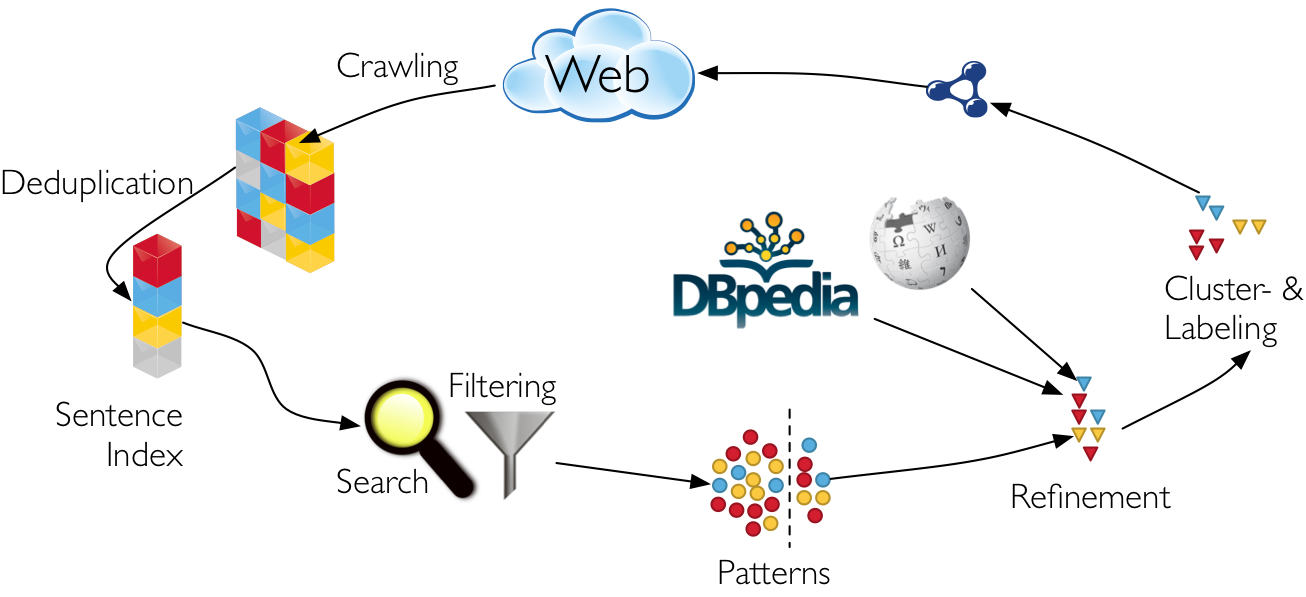
\includegraphics[width=0.9\textwidth]{images/rdflivenews_architecture.png}
	\end{center}
	\caption{Overview of the generic time slice-based stream processing.}
	\label{fig:workflow}
\end{figure}


\subsection{Data Acquisition}
\label{subsec:prerequisites}
Formally, our approach aims to process the output of unstructured data sources $S^i$ by continuously gathering the data streams $D^i$ that they generate.
Each data stream consists of atomic elements $d^i_j$ (in our case sentences).
Let $D^i_{[t, t+d]}$ be the portion of $D^i$ that was emitted by $S^i$ between the times $t$ and $t+d$.
%We call $w$ the emission window (short: window) for $D^i_{[t, t+w]}$.
%We assume that data streams are not necessarily disjoint.
The data gathering begins by iteratively gathering the elements of the streams $D^i_{[t, t+d]}$. from all available sources $S^i$ for a period of time $d$, which we call the \emph{time slice duration}.
For example, this could mean crawling a set of RSS feeds for a duration of 2 hours.
We call $D^i_{[t, t+d]}$ a slice of $D^i$.
We will assume that we begin this process at $t=0$, thus leading to slices $D^i_{[k.d, (k+1).d]}$ with $k \in \mathbb{N}$.
The data gathered from all sources during a time slice duration is called a \emph{time slice}.
%The main content of each data stream $D^i$ for a time slice $t^i$ is extracted and cleaned from HTML markup.
We apply sentence splitting on all slices to generated their elements. %and store the extracted sentences in an index.
%This workflow gets repeated until we reach the end of the time slice.

%%%%%%%%%% THIS IS NOT CLEAR %%%%%%%%%%%%%%%%
%The resulting data is forwarded to the data analysis components of the approach while a new time slice is begun in parallel.
%These components rely on two main resources for the disambiguation and linking of resources:
%(1) The first is created from a Wikipedia dump.
%Again, we apply a sentence boundary disambiguation on all Wikipedia articles and store the resulting sentences in a Lucene index.
%Furthermore we apply the named entity recognition tool and POS tagger from Stanford Core NLP framework%\footnote{\url{http://www-nlp.stanford.edu/software/corenlp.shtml}} 
%on all sentences and store all occurring named entities alongside the sentences and their article URL.
%(2) The second resource is an index of DBpedia.
%We store all URIs from DBpedia with \emph{rdfs:label} and \emph{rdf:type}\footnote{\url{http://www.w3.org/TR/rdf-schema/}} information, a precomputed disambiguation score (see Section~\ref{subsec:pattern_refinement}) and a list of surface forms (``U.S.'' or ``USA'' for the \emph{United States of America}) of each resource.
%This list is compiled by analyzing the \emph{redirect} and \emph{disambiguation} links from Wikipedia as presented in~\cite{MEN11}.
%Note that the extraction of all resources required here is fully automated.

\subsection{Deduplication}
\label{subsec:deduplication}
The aim of the deduplication step is to remove very similar elements from slices before the RDF extraction.
This removal accounts for some Web data streams simply repeating the content of one of several other streams.
Our deduplication approach is based on measuring the similarity of single elements $s_i$ and $s_j$ found in unstructured streams.
Elements of streams are considered to be different iff $qgrams(s_i, s_j) < \theta$, where $\theta \in [0, 1]$ is a similarity threshold and $qgrams(s_i, s_j)$ measures the similarity of two strings by computing the Jaccard similarity of the trigrams they contain.
Given that the number of stream items to deduplicate can be very large, we implemented the following two-step approach:
For each slice $D^i_{[k.d, (k+1)d]}$, we first deduplicate the elements $s^i_j$ within $D^i_{[k.d, (k+1)d]}$.
This results in a duplicate-free data stream $\Delta^i_{[k.d, (k+1)d]} = \{d^i_j:  (d^i_j \in D^i_{[k.d, (k+1)d]}) \wedge (\forall s^i_k \in D^i_{[k.d, (k+1)d]}\ \exists d^i_j \in \Delta^i_{[k.d, (k+1)d]}\ qgrams(s^i_k, d^i_j) \geq \theta) \wedge (\forall d^i_j, d^i_k \in \Delta^i_{[k.d, (k+1)d]}\ qgrams(d^i_k, d^i_j) < \theta)\}$.
The elements of $\Delta^i_{[k.d, (k+1)d]}$ are then compared to all other elements of the $w$ previous deduplicated streams $\Delta^i_{[(k-1).d, kd]}$ to $\Delta^i_{[(k-w).d, (k-w+1)d]}$, where $w$ is the size of the deduplication window.
Only $\Delta^i_{[k.d, (k+1)d]}$ is used for further processing.
To ensure the scalability of the deduplication step, we are using deduplication algorithms implemented in the LIMES framework~\cite{DBLP:journals/jodsn/Ngomo12}.
Table~\ref{tab:dedup} gives an overview of the number of unique data stream items in our dataset when using different deduplication thresholds.

%%\todo{SH: I still can not understand, what an iteration in table 1 is?}
%\setlength{\tabcolsep}{6pt}
%\begin{table}[tb]
%	\centering
%	\caption{Number of non-duplicate sentences in 1\% of the data extracted from 1457 RSS feeds within a window of 10 time slices (2h each). The second column shows the original number of sentences without duplicate removal.}       
%	\label{tab:dedup}
%    \begin{tabular}{ccccccc} 
%        \toprule
%		Time Slice & No deduplication & $\theta = 1.0$ & $\theta = 0.95$ & $\theta = 0.9$ & $\theta = 0.85$ & $\theta = 0.8$ \\ \midrule
%		1 & 2997 & 2764 & 2764 & 2759 & 2754 & 2753 \\
%		5 & 3047 & 2335 & 2334 & 2327 & 2320 & 2315 \\
%		10 & 3113 & 2033 & 2040 & 2022 & 2015 & 2010 \\
%		15 & 2927 & 1873 & 1868 & 1866 & 1864 & 1855 \\
%		20 & 3134 & 1967 & 1966 & 1949 & 1945 & 1941 \\
%		25 & 3065 & 1936 & 1932 & 1924 & 1919 & 1915 \\
%		30 & 3046 & 1941 & 1940 & 1933 & 1928 & 1924 \\\bottomrule
%		%35 & 2991 & 1877 & 1872 & 1866 & 1861 & 1856 \\ \bottomrule
%    \end{tabular}
%\end{table}

\subsection{Pattern Search and Filtering}
\label{subsec:pattern_search}
%sh I moved the definition of 
In order to find patterns we first apply Named Entity Recognition (NER) and Part of Speech (POS) tagging on the deduplicated sentences.
\NAME{} can use two different ways to extract patterns from annotated text.
The POS tag method uses \emph{NNP} and \emph{NNPS}\footnote{All POS tags can be found in the Penn Treebank Tagset.} tagged tokens to identify a relation's subject and object, whereas the Named Entity Tag method relies on \emph{Person}, \emph{Location}, \emph{Organization} and \emph{Miscellaneous} tagged tokens.
% NNPS is the plural of NNP
% \todo[inline]{Lorenz: What is S, I guess the sentence? Why not only NNP?}
In an intermediate step all consecutive POS and NER tags are merged.
An unrefined \NAME{} pattern $p$ is now defined as a pair $p = (\theta, \mathcal{S_\theta})$, where $\theta$  is the natural language representation (NLR) of $p$ and $\mathcal{S_\theta} = \{(s_i,o_i) : i \in \mathbb{N}; 1 \le i \le n\}$ is the support set of $\theta$, a set of the subject and object pairs. 
For example the sentence:
\vspace*{4pt}\\
{\noindent\small David/NNP hired/VBD John/NNP ,/, former/JJ manager/NN of/IN ABC/NNP ./.}
\vspace*{4pt}\\
would result in the patterns:
\vspace*{6pt}\\
\indent$p_1 = (\:[hired], \{(David,\:John)\}$ and \newline
\indent$p_2 = ([,\;former\;manager\;of], \{(John,\;ABC)\})$.
\vspace*{4pt}\\
%Please note that weekdays like ``Monday'' are not allowed as subject or object of a pattern, since days are not 
%Additionally, this step is performed in parallel.
After the initial pattern acquisition step, we filter all patterns to improve their quality.
We discarded all patterns that did not match these criteria:
The pattern should (1) contain at least a verb or a noun, (2) contain at least one salient word (i.e. a word that is not a stop word), (3) not contain more than one non-alpha-numerical character (except ", ' `") and (4) be shorter than 50 characters.
%\begin{enumerate}[(1)]
    %\item contain at least a verb or a noun,
    %\item contain at least one salient word (i.e. a word that is not a stop word), 
    %\item not contain more than one non-alpha-numerical character (except ", ' `"), 
    %\item be shorter than 50 characters.
%\end{enumerate}
% We created a set of filtering criteria, like patterns need to contain either a verb or a noun, need to contain at least one non stop word, shall  and need to be shorter than 50 characters etc.
Since the resulting list still contains patterns of low quality, we first sort it by the number of elements of the support set $\mathcal{S}_\theta$ and solely select the top 1\% for pattern refinement to ensure high quality.

\subsection{Pattern Refinement}
\label{subsec:pattern_refinement}%\todo[inline]{Lorenz: In general, can we expect that the reader knows RDF and the prefixes/relations?}
The goal of this step is to find a suitable \emph{rdfs:range} and \emph{rdfs:domain} as well as to disambiguate the support set of a given pattern.
To achieve this goal we first try to find an URI for the subjects and objects in the support set of $p$ by matching the pairs to entries in a knowledge base.
With the help of those URIs we can query the knowledge base for the classes (\emph{rdf:type}) of the given resources and compute a common \emph{rdfs:domain} for the subjects of $p$ and \emph{rdfs:range} for the objects respectively. 
A refined \NAME{} pattern \texttt{$p_r$} is now defined as a quadruple $p_r = (\theta, \mathcal{S_\theta}', \delta, \rho)$, where $\theta$ is the natural language representation, $\mathcal{S_\theta}'$ the disambiguated support set, $\delta$ the \emph{rdfs:domain} and $\rho$ the \emph{rdfs:range} of $p_r$. 
%The pattern refinement is carried out in parallel.

To find the URIs of each subject-object pair $(s,o) \in \mathcal{S_\theta}$ we first try to complete the entity name.
This step is necessary and beneficial because entities usually get only written once in full per article.
For example the newly elected president of the United States of America might be referenced as ``President Barack Obama'' in the first sentence of a news entry and subsequently be referred to as ``Obama''.
In order to find the subjects' or objects' full name, we first select all named entities $e \in \mathcal{E}_a$ of the article the pair $(s,o)$ was found in. We then use the longest matching substring between $s$ (or $o$) and all elements of $\mathcal{E}_a$ as the name of $s$ or $o$ respectively.
Additionally we can filter the elements of $\mathcal{E}_a$ to contain only certain NER types.
Once the complete names of the entities are found, we can use them to generate a list of URI candidates $\mathcal{C}_{uri}$.
This list is generated with the help of a query for the given entity name on a list of surface forms (e.g. ``U.S.'' or ``USA'' for the \emph{United States of America}), which was compiled by analyzing the \emph{redirect} and \emph{disambiguation} links from Wikipedia as presented in~\cite{MEN11}.
Each URI candidate $c \in \mathcal{C}_{uri}$ is now evaluated on four different features and the combined score of those features is used to rank the candidates and choose the most probable URI for an entity.
The first feature is the \emph{Apriori}-score $a(c)$ of the URI candidate $c$, which is calculated beforehand for all URIs in the knowledge base by analyzing the number of inbound links of $c$ by the following formula: $a(c) = \log(inbound(c) + 1)$.
The second and third features are based on the context information found in the Wikipedia article of $c$ and the news article text $(s,o)$ was found in.
For the \emph{global context}-score $c_g$ we apply a co-occurrence analysis of the entities $\mathcal{E}_a$ found in the news article and the entities $\mathcal{E}_w$ found in the Wikipedia article of $c$.
The \emph{global context}-score is now computed as $c_g(\mathcal{E}_a,\mathcal{E}_w) = {|\mathcal{E}_a \cap\mathcal{E}_w|}\:/\:{|\mathcal{E}_a \cup \mathcal{E}_w|}$. 
The \emph{local context}-score $c_l$ is the number of mentions of the second element of the pair $(s,o)$, $o$ in the case of $s$ and vice versa, in $\mathcal{E}_w$.
The last feature to determine a URI for an entity is the maximum string similarity $sts$ between $s$ (or $o$) and the elements of the list of surface forms of $c$.
We used the qgram distance\footnote{\url{http://sourceforge.net/projects/simmetrics/}} as the string similarity metric.
We normalize all non-$[0,1]$ features ($c_g, c_l, a$) by applying a minimum-maximum normalization of the corresponding scores for $\mathcal{C}_{uri}$ and multiply it with a weight parameter which leads to the overall URI score:
\begin{displaymath}
	c(s,o,uri) = \dfrac{\dfrac{\alpha a}{a_{max}} + \dfrac{\beta c_g}{c_{g_{max}}} + \dfrac{\gamma c_l}{c_{l_{max}}} + \delta sts}{4}
\end{displaymath}
If the URI's score is above a certain threshold $\lambda \in [0, 1]$ we use it as the URI for $s$, otherwise we create a new URI.
Once we have computed the URIs for all pairs $(s,o) \in \mathcal{S_\theta}$ we determine the most likely \emph{domain} and \emph{range} for $p_r$.
This is done by analyzing the \emph{rdf:type} statements returned for each subject or object in $\mathcal{S_\theta}$ from a background knowledge base.
Since the DBpedia ontology is designed in such a way, that classes do only have one super-class, we can easily analyze its hierarchy.
We implemented two different determination strategies for analyzing the class hierarchy.
The first strategy, dubbed ``most general'', selects the highest class in the hierarchy for each subject (or object) and uses the most occurring class as \emph{domain} or \emph{range} of $p_r$.
The second strategy, dubbed ``most specific'', works similar to the ``most general'' strategy with the difference that it uses the most descriptive class to select the \emph{domain} and \emph{range} of $p_r$.

\subsection{Pattern Similarity and Clustering}
\label{subsec:pattern_clustering}
In order to cluster patterns according to their meaning, we created a set of similarity measures.
A similarity measure takes two patterns $p_1$ and $p_2$ as input and outputs the similarity value $s(p_1,p_2) \in [0,1]$.
As a baseline we implemented a qgram measure, which calculates the string similarity between all non stop words of two patterns.
Since this baseline measure fails to return a high similarity for semantically related, but not textually similar patterns like ``'s attorney ,'' and ``'s lawyer ,'' we also implemented a Wordnet measure.
As a first step the Wordnet similarity measure filters out the stop words of $p_1$ and $p_2$ and applies the Stanford lemmatizer on the remaining tokens.
Subsequently, for all token combinations of $p_1$ and $p_2$, we apply a Wordnet Similarity metric (Path~\cite{conf/aaai/PedersenPM04}, Lin~\cite{similarity-lin} and Wu \& Palmer~\cite{conf/acl/WuP94}) and select the maximum of all comparisons as the similarity value $s(p_1,p_2)$.
As a final similarity measure we created a Wordnet and string similarity measure with the help of a linear combination from the before-mentioned metrics. 
In this step we also utilize the \emph{domain} and \emph{range} of $p_r$.
If this feature is enabled, a similarity value between two patterns $p_1$ and $p_2$ can only be above 0, iff $\{\delta_{p_1},\rho_{p_1}\} \setminus \{\delta_{p_2},\rho_{p_2}\} = \emptyset$.

%Note that the runtime complexity of the similarity generation is $\mathcal{O}(n^2)$, which made it necessary to limit the number of patterns used in the similarity generation, as well as to implement this step in parallel. 

The result of the similarity computation can be regarded as a similarity graph $G = (V, E, \omega)$, where the vertices are patterns and the weight $\omega(p_1, p_2)$ of the edge between two patterns is the similarity of these patterns. 
Consequently, unsupervised machine learning and in particular graph clustering is a viable way of finding groups of patterns that convey similar meaning.
We opted for using the BorderFlow clustering algorithm~\cite{DBLP:conf/cicling/NgomoS09} as it is parameter-free and has already been used successfully in diverse applications including clustering protein-protein interaction data and queries for SPARQL benchmark creation~\cite{DBLP:conf/semweb/MorseyLAN11}.
For each node $v \in V$, the algorithm begins with an initial cluster $X$ containing only $v$. 
Then, it expands $X$ iteratively by adding nodes from the direct neighborhood of $X$ to $X$ until $X$ is node-maximal with respect to the border flow ratio described in~\cite{DBLP:conf/semweb/MorseyLAN11}. 
The same procedure is repeated over all nodes. 
As different nodes can lead to the same cluster, identical clusters (i.e., clusters containing exactly the same nodes) that resulted from different nodes are subsequently collapsed to one cluster. 
The set of collapsed clusters and the mapping between each cluster and the nodes that led to it are returned as result.

\subsection{Cluster Labeling and Merging}
\label{subsec:cluster_labeling_and_merging}
Based on the clusters $\mathcal{C}$ obtained through the clustering algorithm, this step selects descriptive labels for each cluster $c_i\in\mathcal{C}$, which can afterwards be used to merge the clusters.
In the current version, we apply a straightforward majority voting algorithm, i.e. for each cluster $c_i$, we select the most frequent natural language representation $\theta$ (stop words removed) occurring in the patterns of $c_i$.
Finally, we use the representative label of the clusters to merge them using a string similarity and WordNet based similarity measure.
This merging procedure can be applied repeatedly to further reduce the number of clusters, but taking into account that those similarity measures are not transitive, we are currently only 
running it once, as we're more focused on accuracy.

\subsection{Mapping to RDF and Publication on the Web of Data}
\label{subsec:rdf_publication}
To close the circle of the round-trip pipeline of \NAME, the following prerequisite steps are required to re-publish the extraction results in a sensible way:
\begin{enumerate}
 \item The facts and properties contained in the internal data structure of our tool have to be mapped to OWL.
 \item Besides the extracted factual information several other aspects and meta data are interesting as well, such as extraction and publication data and provenance links to the text the facts were extracted from.
 \item URIs need to be minted to provide the extracted triples as linked data. 
\end{enumerate}

\textbf{Mapping to OWL.} Each cluster $c_i \in \mathcal{C}$ represents an \emph{owl:ObjectProperty} $prop_{c_i}$.
The \emph{rdfs:domain} and \emph{rdfs:range} of $prop_{c_i}$ is determined by a majority voting algorithm with respect to $\delta$ and $\rho$ of all $p_r \in \mathcal{C}$.
The \emph{skos:prefLabel}\footnote{\url{http://www.w3.org/2004/02/skos/}} of $prop_{c_i}$ is the label determined by the cluster labeling step and all other NLRs of the patterns in $c_i$ get associated with $prop_{c_i}$ as \emph{skos:altLabels}.
For each subject-object pair in $\mathcal{S_\theta}'$ we produce a triple by using $prop_{c_i}$ as predicate and by assigning learned entity types from DBpedia or \emph{owl:Thing}. 

\textbf{Provenance tracking with NIF.} Besides converting the extracted facts from the text, we are using the current draft of the NLP Interchange Format (NIF) Core ontology\footnote{\url{http://persistence.uni-leipzig.org/nlp2rdf/ontologies/nif-core#}} to serialize the following information in RDF: the sentence the triple was extracted from, the extraction date of the triple, the link to the source URL of the data stream item and the publication date of the item on the stream.
Furthermore, NIF allows us to link each element of the extracted triple to its origin in the text for further reference and querying. 

NIF is an RDF/OWL based format to achieve interoperability between language tools, annotation and resources. NIF offers several URI schemes to create URIs for strings, which can then be used as subjects for annotation. We employ the NIF URI scheme, which is grounded on URI fragment identifiers for text (RFC 5147\footnote{\url{http://tools.ietf.org/html/rfc5147}}). 
NIF was previously used by NERD~\cite{EURECOM+3675} to link entities to text.  
For our use case, we extended NIF in two ways: 
(1) we added the ability to represent extracted triples via the ITS 2.0 / RDF Ontology\footnote{\url{http://www.w3.org/2005/11/its/rdf#}}. 
\emph{itsrdf:taPropRef} is an \emph{owl:AnnotationProperty} that links the NIF String URI to the \emph{owl:ObjectProperty} by \NAME. 
The three links from the NIF String URIs ($str_1$, $str_2$, $str_3$) to the extracted triple ($s$, $p$, $o$) itself make it well traceable and queryable: 
$str_1$ $\mapsto$ $s$, $str_2$  $\mapsto$  $p$, $str_3$  $\mapsto$  $o$,  $s$  $\mapsto$  $p$ $\mapsto$ $o$ .
An example of NIF RDF serialization is shown in Listing~\ref{lst:rdf_extraction}.
(2) Although \cite{EURECOM+3675} already suggested the minting of new URIs, a concrete method for doing so was not yet researched. 
In \NAME{} we use the source URL of the data stream item to re-publish the facts for individual sentences as linked data. 
We strip the scheme component (http://) of the source URL and percent encode the ultimate part of the path and the query component\footnote{\url{http://tools.ietf.org/html/rfc3986#section-3}} and add the md5 encoded sentence to produce the following URI:
{\small \begin{verbatim}
http://rdflivenews.aksw.org/extraction/ + example.com:8042/over/ +
    urlencode(there?name=ferret) + / + md5(`sentence`)
\end{verbatim}}
\lstinputlisting[caption=Example RDF extraction of \NAME{},label=lst:rdf_extraction, language=ttl]{listings/rdf_extraction_nif2.tex}

\textbf{Republication of RDF.} The extracted triples are hosted on: \url{http://rdflivenews.aksw.org}. 
The data for individual sentences is crawlable via the file system of the Apache2 web server. 
We assume that source URLs only occur once in a stream when the document is published and the files will not be overwritten. 
Furthermore, the extracted properties and entities are available as linked data at \emph{http://rdflivenews.aksw.org/\{ontology|resource\}/\$name} and they can be queried via SPARQL at \url{http://rdflivenews.aksw.org/sparql}. 

%TODO query idea: All subjects of type   ?proRef, 

\subsection{Linking}
\label{subsec:mapping_to_dbpedia}
The approach described above generates a set of properties with several labels. 
In our effort to integrate this data source into the Linked Open Data Cloud, we use the deduplication approach proposed in Section~\ref{subsec:deduplication} to link our set of properties to existing knowledge bases (e.g., DBpedia).
To achieve this goal, we consider the set of properties we generated as set of source instances $S$ while the properties of the knowledge base to which we link are considered to be a set of target $T$.
Two properties $s \in S$ and $t \in T$ are linked iff $trigrams(s, t) \geq \theta_p$, where $\theta_p \in [0, 1]$ is the property similarity threshold.
 
\section{Evaluation}
\label{sec:evaluation}
The aim of our evaluation was to answer four questions.
First, we aimed at testing how well \NAME{} is able to disambiguate found entities. 
Our second goal was to determine if the proposed similarity measures can be used to cluster patterns with respect to their semantic similarity.
Third, we wanted to evaluate the quality of the RDF extraction and linking.
Finally, we wanted to measure if all computational heavy tasks can be applied in real-time, meaning the processing of one iteration takes less time than its compilation.

For this evaluation we used a list of 1457 RSS feeds as compiled in \cite{GOLDHAHN12.327}.
%\todo{something is missing after wolrd,}
This list includes all major worldwide newspapers and a wide range of topics, e.g. \emph{World}, \emph{U.S.}, \emph{Business}, \emph{Science} etc.
We crawled this list for 76 hours, which resulted in a corpus, dubbed \emph{100\%} of 38 time slices of 2 hours and 11.7 million sentences.
The average number of sentences per feed entry is approximately 26.5 and there are 3445 articles on average per time slice.
Additionally we created two subsets of this corpus by randomly selecting 1\% and 10\% of the contained sentences.
All evaluations were carried out on a MacBook Pro with a quad-core Intel Core i7 (2GHz), a solid state drive and 16 GB of RAM.
\subsection{URI Disambiguation}
To evaluate the URI disambiguation we created a gold standard manually.
We took the 1\% corpus, applied deduplication with a window size of 40 (contains all time slices) and a threshold of 1 (identical sentences), which resulted in a set of 69884 unique sentences.
On those sentences we performed the pattern extraction with part of speech tagging as well as filtering.
In total we found 16886 patterns and selected the Top 1\%, which have been found by 1729 entity pairs.
For 473 of those entity pairs we manually selected a URI for subject and object.
This resulted in an almost equally distributed gold standard with 456 DBpedia and 478 \NAME{} URIs.
We implemented a hill climbing approach with random initialization to optimize the parameters (see Section~\ref{subsec:pattern_refinement}).
The precision of our approach is the ratio between correctly found URIs for subject and object to the number of URIs above the threshold $\lambda$ as shown in Equation~\ref{eq:p}.
The recall, shown in Equation~\ref{eq:r}, is determined by the ratio between the number of correct subject and object URIs and the total number of subjects and objects in the gold standard.
The $F_1$ measure is determined as usual by: $F_1=2 \cdot \frac{P \cdot R}{P + R}$.
We optimized our approach for precision since we can compensate a lower recall and could achieve a precision of \textbf{85.01\%} where the recall is \textbf{40.69\%} and the resulting $F_1$ is \textbf{55.03\%}.
The parameters obtained through the hill-climbing search indicate that the \emph{Apriori}-score is the most influential parameter (1.0), followed by \emph{string-similarity} (0.78), \emph{local-context} (0.6), global context (0.45) and a URI score threshold of 0.61.
If we optimize for $F_1$, we were able to achieve a $F_1$ measure of \textbf{66.49\%} with a precision of \textbf{67.03\%} and a recall of \textbf{65.95\%}.

%The URI disambiguation suffers from a medium recall.
For 487 out of the 934 URI in the gold standard no confident enough URI could be found.
The most problems occured for DBpedia URIs which could not be determined in 305 cases, in comparison to 182 URIs for newly created resources.
Additionally, for 30 resources \NAME{} created new URIs where DBpedia URIs should be used and in 0 cases a DBpedia URI was used where a new resource should be created.
The reason for those mistakes are tagging errors, erroneous spellings and missing context information.
For example Wikipedia has 97 disambiguations for ``John Smith'' which can not be disambiguated without prior knowledge.

% \todo{somebody please review the paragraph below}
% \todo{sh: I read it and rewrote parts of it, please verify}
We used AIDA \cite{HoYoBo2011} to compare our results with a state-of-the-art NED algorithm. 
We configured AIDA with the Cocktailparty setup, which defines the recommended configuration options of AIDA.
AIDA achieved an accuracy of 0.57, i.e. 57\% of the identifiable entities were correctly disambiguated.
The corpus described above provides a difficult challenge due to the small disambiguation contexts and is limited to graphs evolving from two named entities per text.
AIDA tries to build dense sub-graphs in a greedy manner in order to perform correct disambiguation. 
This algorithm would profit from a bigger number of entities per text.
The drawback is AIDA needs 2 minutes to disambiguate 25 sentences.
Overall, AIDA performs well on arbitrary entities.


\vspace{1em}
\noindent\begin{minipage}{.5\linewidth}
\begin{equation}
	\label{eq:p}
  P = \frac{|{s_{uri_c}}|+|{o_{uri_c}}|}{|s_{uri}|+|o_{uri}|}
\end{equation}
\end{minipage}%
\begin{minipage}{.5\linewidth}
\begin{equation}
	\label{eq:r}
  R = \frac{|{s_{uri_c}}|+|{o_{uri_c}}|}{2\cdot|GS|}
\end{equation}
\end{minipage}

\subsection{Pattern Clustering}
To evaluate the similarity generation as well as the clustering algorithm we relied on the measures Sensitivity, Positive Predictive Value (PPV) and Accuracy.
We used the adaptation of those measures as presented in \cite{journals/bmcbi/BroheeH06} to measure the match between a set of pattern mappings\footnote{A pattern mapping maps NLRs to RDF properties.} from the gold standard and a clustering result.
The gold standard was created by clustering the patterns as presented in the previous section manually.
This resulted in a list of 25 clusters with more than 1 pattern and 54 clusters with 1 pattern.
Since cluster with a size of 1 would skew our evaluation into unjustified good results, we excluded them from this evaluation.

\textbf{Sensitivity.} With respect to the clustering gold standard, we define sensitivity as the fraction of patterns of pattern mapping $i$ which are found in cluster $j$.
In $Sn_{i,j} = T_{i,j}/N_i$, $N_i$ is the number of patterns belonging to pattern mapping $i$.
We also calculate a pattern mapping-wise sensitivity $Sn_{pm_i}$ as the maximal fraction of patterns of pattern mapping $i$ assigned to the same cluster. 
$Sn_{pm_i} = max^m_{j=1}Sn_{i,j}$ reflects the coverage of pattern mapping $i$ by its best-matching cluster.
To characterize the general sensitivity of a clustering result, we compute a clustering-wise sensitivity as the weighted average of $Sn_{pm_i}$ over all pattern mappings:
$Sn=\frac{\sum_{i=1}^nN_iSn_{pm_i}}{\sum_{i=1}^nN_i}$.

\textbf{Positive Predictive Value.} The positive predictive value is the proportion of members of cluster $j$ which belong to pattern mapping $i$, relative to the total number of members of this cluster assigned to all pattern mappings.
$PPV_{i,j} = T_{i,j} / \sum_{i=1}^n T_{i,j} =T_{i,j} /T_{.j}$ \\
$T_{.j}$ is the sum of column $j$.
We also calculate a cluster-wise positive predictive value $PPV_{cl_j}$, which represents the maximal fraction of patterns of cluster $j$ found in the same annotated pattern mapping.
$PPV_{cl_j} =max^n_{i=1} PPV_{i,j}$ reflects the reliability with which cluster $j$ predicts that a pattern belongs to its best-matching pattern mapping.
To characterize the general PPV of a clustering result as a whole, we compute a clustering-wise PPV as the weighted average of $PPV_{cl_j}$ over all clusters: 
$PPV=\frac{\sum_{j=1}^mT_{.j}PPV_{cl_j}}{\sum_{j=1}^mT_{.j}}$.

\textbf{Accuracy.} The geometric accuracy (Acc) indicates the tradeoff between sensitivity and positive predictive value. It is obtained by computing the geometrical mean of the $Sn$ and the $PPV$:
$Acc= \sqrt{Sn\cdot PPV}$.

We evaluated the three similarity measures with respect to the underlying WordNet similarity metric (see Section~\ref{subsec:pattern_clustering}).
Furthermore we varied the clustering similarity threshold between 0.1 and 1 with a 0.1 step size.
% evaluation showed that this does not make a difference: and evaluated the domain and range restrictions in the similarity generation step.
% i dont know why this is the case
In case of the qgram and WordNet similarity metric we performed a grid search on the WordNet and qgram parameter in $[0,1]$ with a step size of 0.05.
We achieved the best configuration with the qgram and WordNet similarity metric with an accuracy of \textbf{82.45\%}, a sensitivity of \textbf{71.17\%} and a positive predictive value of \textbf{95.51\%}.
The best WordNet metric is Lin, the clustering threshold 0.3 and the qgram parameter is with 0.45 significantly less influential than the WordNet parameter with 0.75.
As a reference value, the plain WordNet similarity metric achieved an accuracy of 78.86\% and the qgram similarity metric an accuracy of 69.1\% in their best configuration.

\subsection{RDF Extraction and Linking}
To assess the quality of the RDF data extracted by \NAME{}, we sampled the output of our approach and evaluated it manually.
We generated five different evaluation sets.
Each set may only contain triples with properties of clusters having at least $i = 1 \dots 5$ patterns.
We selected 100 triples (if available) randomly for each test set.
As the results in Table~\ref{tab:rdfacc} show, we achieve high accuracy on subject and object disambiguation.
As expected, the precision of our approach grows with the threshold for the minimal size of clusters.
This is simply due to the smaller clusters having a higher probability of containing outliers and thus noise.

\setlength{\tabcolsep}{2pt}
\begin{table}[!htb]
    \begin{minipage}[t]{.47\linewidth}
    \vspace{0pt}
   	\caption{	\label{tab:rdfacc}
Accuracy of RDF Extraction for subject (S), predicates (P) and objects (O) on 1\% dataset with varying cluster sizes $E_i$.}       

        \begin{tabular}{>{\centering\arraybackslash}p{1.4cm}ccccc} 
        \toprule
		$E_i$         &  1       &  2       &  3       &  4       &    5      \\ \midrule
		$S_{Acc}$           &  0.81  &  0.88  &  0.86  &  0.857  &  0.804 \\ 
		$P_{Acc}$           &  0.86  &  0.89  &  0.90  &  0.935  &  1.00 \\ 
       $O_{Acc}$           &  0.93  &  0.91  &  0.90  &  0.948  &  0.941 \\ 
		$Total_{Acc}$       &  0.86  &  0.892  &  0.885  &  0.911  &  0.906 \\ 
		$|E_i|$             &  100     &  100     &  100     &  77      &  51 \\ 
		$|P| \in |E_i|$     &  28      &  22      &  12      &  6       &  1 \\ \bottomrule
    \end{tabular}
    \end{minipage}%
        \hspace{0.5em}
        \setlength{\tabcolsep}{1pt}
    \begin{minipage}[t]{.47\linewidth}
        \vspace{0pt}
        	
        	   	\caption{\label{tab:dedup}Number of non-duplicate sentences in 1\% of the data extracted from 1457 RSS feeds within a window of 10 time slices (2h each). The second column shows the original number of sentences without duplicate removal.}  

    \begin{tabular}{>{\centering\arraybackslash}p{1cm}>{\centering\arraybackslash}p{1.5cm}ccc} 
        \toprule
		Time Slice & No deduplication & $\theta = 1.0$ & $\theta = 0.95$ & $\theta = 0.9$ \\ \midrule %& $\theta = 0.85$ & $\theta = 0.8$ \\ \midrule
		1 & 2997 & 2764 & 2764 & 2759 \\
		5 & 3047 & 2335 & 2334 & 2327 \\
		10 & 3113 & 2033 & 2040 & 2022   \\
		15 & 2927 & 1873 & 1868 & 1866   \\
		20 & 3134 & 1967 & 1966 & 1949   \\
		25 & 3065 & 1936 & 1932 & 1924   \\
		30 & 3046 & 1941 & 1940 & 1933   \\\bottomrule
		%1 & 2997 & 2764 & 2764 & 2759 & 2754 & 2753 \\
		%5 & 3047 & 2335 & 2334 & 2327 & 2320 & 2315 \\
		%10 & 3113 & 2033 & 2040 & 2022 & 2015 & 2010 \\
		%15 & 2927 & 1873 & 1868 & 1866 & 1864 & 1855 \\
		%20 & 3134 & 1967 & 1966 & 1949 & 1945 & 1941 \\
		%25 & 3065 & 1936 & 1932 & 1924 & 1919 & 1915 \\
		%30 & 3046 & 1941 & 1940 & 1933 & 1928 & 1924 \\\bottomrule
		%35 & 2991 & 1877 & 1872 & 1866 & 1861 & 1856 \\ \bottomrule
    \end{tabular}
    \end{minipage} 
\end{table}


\setlength{\tabcolsep}{3pt}
\begin{table}[tb]
	\centering
	\caption{\label{tab:linking}Example for linking between \NAME{} and DBpedia.}       
    \begin{tabular}{llp{6cm}} 
       \toprule
		\NAME{}-URI &  DBpedia-URI       &  Sample of cluster\\ \midrule
		rlno:directorOf & dbo:director & [manager], [, director of], [, the director of]\\
		rlno:spokesperson &  dbo:spokesperson &  [, a spokeswoman for], [spokesperson],\newline [, a spokesman for]\\
		rlno:attorney & --- & ['s attorney ,], ['s lawyer ,], [attorney]\\
    \bottomrule
    \end{tabular}
\end{table}
 The results of the linking with DBpedia (see Table~\ref{tab:linking}) showed the mismatch between the relations that occur in news and the relations designed to model encyclopedic knowledge.
While some relations such as \texttt{dbo:director} are used commonly in news streams and in the Linked Data Cloud, relations with a more volatile character such as \texttt{rlno:attorney} which appear frequently in news text are not mentioned in DBpedia. 
\subsection{Scalability}
In order to perform real-time RDF extraction, the processing of the proposed pipeline needs to be done in less time than its acquisition requires.
This also needs to be true for a growing list of RSS feeds.
Therefore, we analyzed the time each module needed in each iteration and compared these values between the three test corpora.
An early approximation of this evaluation implied that the pipeline indeed was not fast enough, which led to the parallelization of the pattern refinement and similarity generation. 
The results of this evaluation can be seen in Figure~\ref{fig:speed}.
\begin{figure*}[tb]
	\begin{center}
		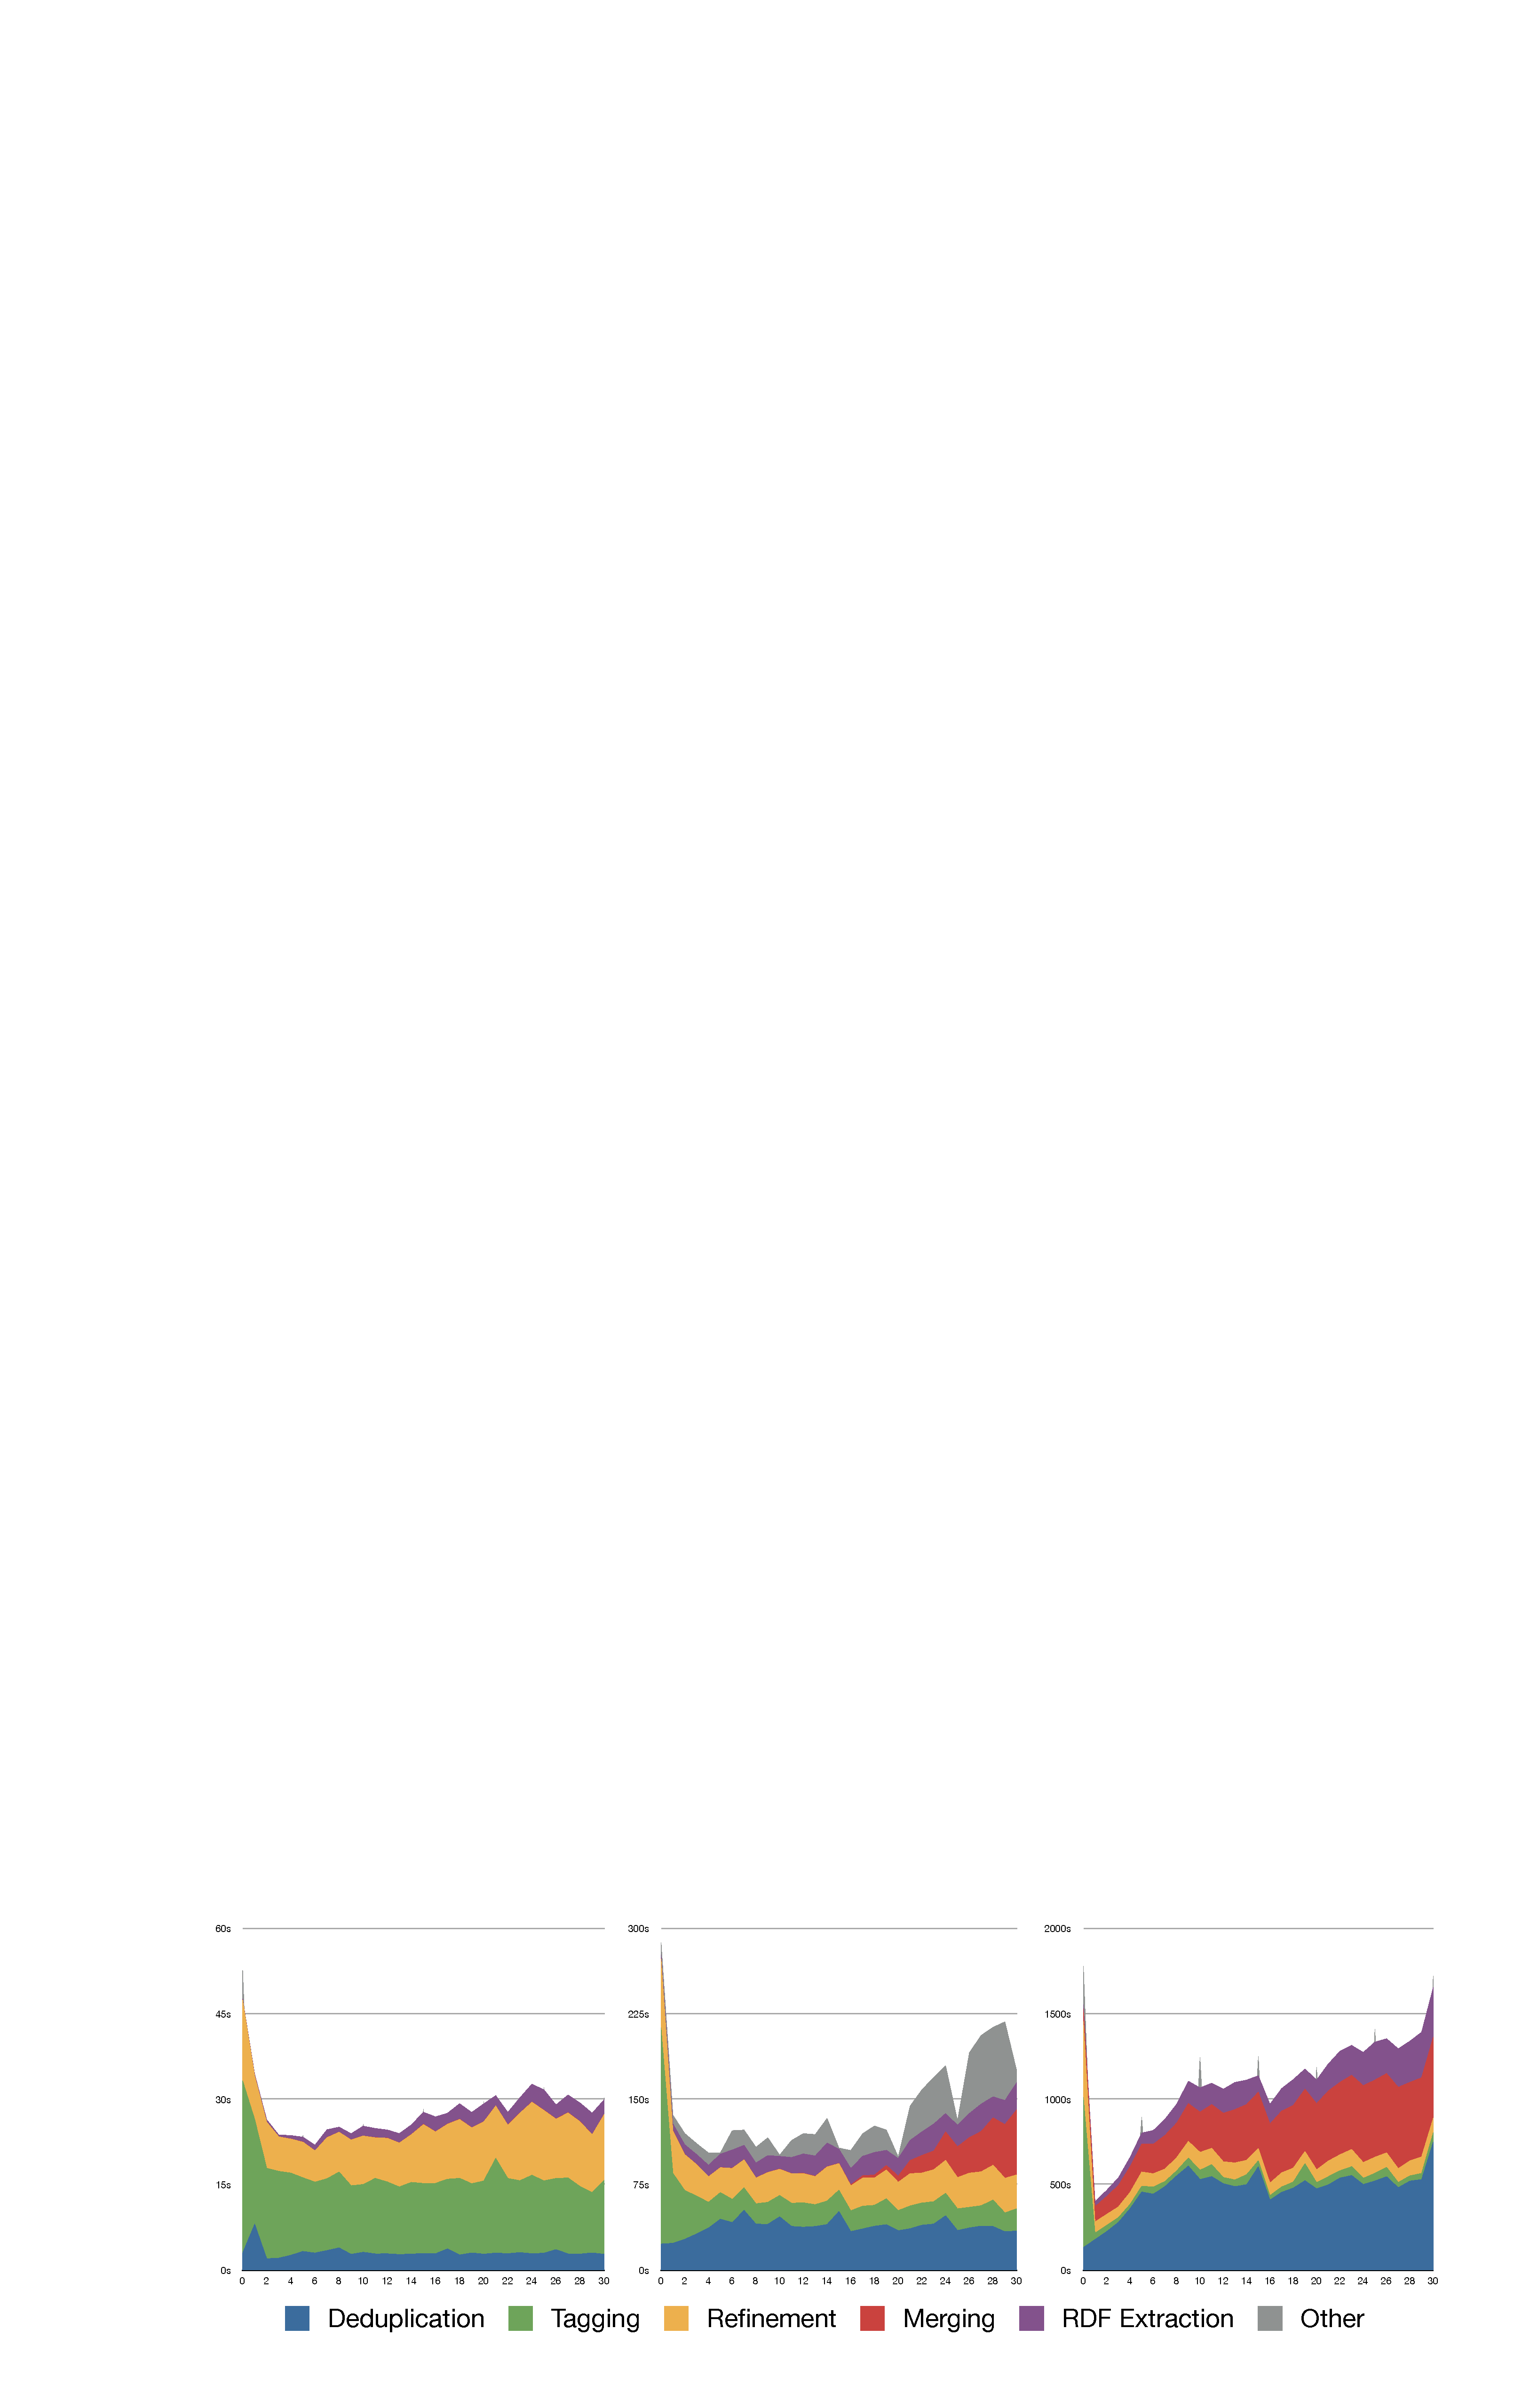
\includegraphics[width=\textwidth]{images/speed.pdf}
	\end{center}
	\caption{Runtimes for different components and corpora (1\% left, 10\% middle, 100\% right) per iteration.}
	\label{fig:speed}
\end{figure*}
With an average time slice processing time of about 20 minutes for the 100\% corpus (2.2 minutes for 10\% and 30s for 1\%), our approach is clearly fit to handle up to 1500 RSS and more.
The spike in the first iteration results out of the fact that RSS feeds contain the last $n$ previous entries, which leads to a disproportional large first time slice.
The most time consuming modules are the deduplication, tagging and cluster merging.
To tackle these bottlenecks we can for example parallelize sentence tagging and the deduplication.

The results of the growth evaluation for patterns until iteration 30 can be seen in Figure~\ref{fig:patterns}.
The number of patterns grows with the factor of 3 from 1\% to 10\% and 10\% to 100\% corpora.
Also, the number of patterns found by more than one subject-object pair increases approximately by factor 2.
Additionally we observed a linear growth for all patterns (also for patterns with $|\mathcal{S}_\theta'| > 1$) and 100\% showing the highest growth rate with a factor 2.5 over 10\% and 4.8 over 10\%.

\begin{figure}
\centering
\begin{minipage}{.49\textwidth}
  \centering
  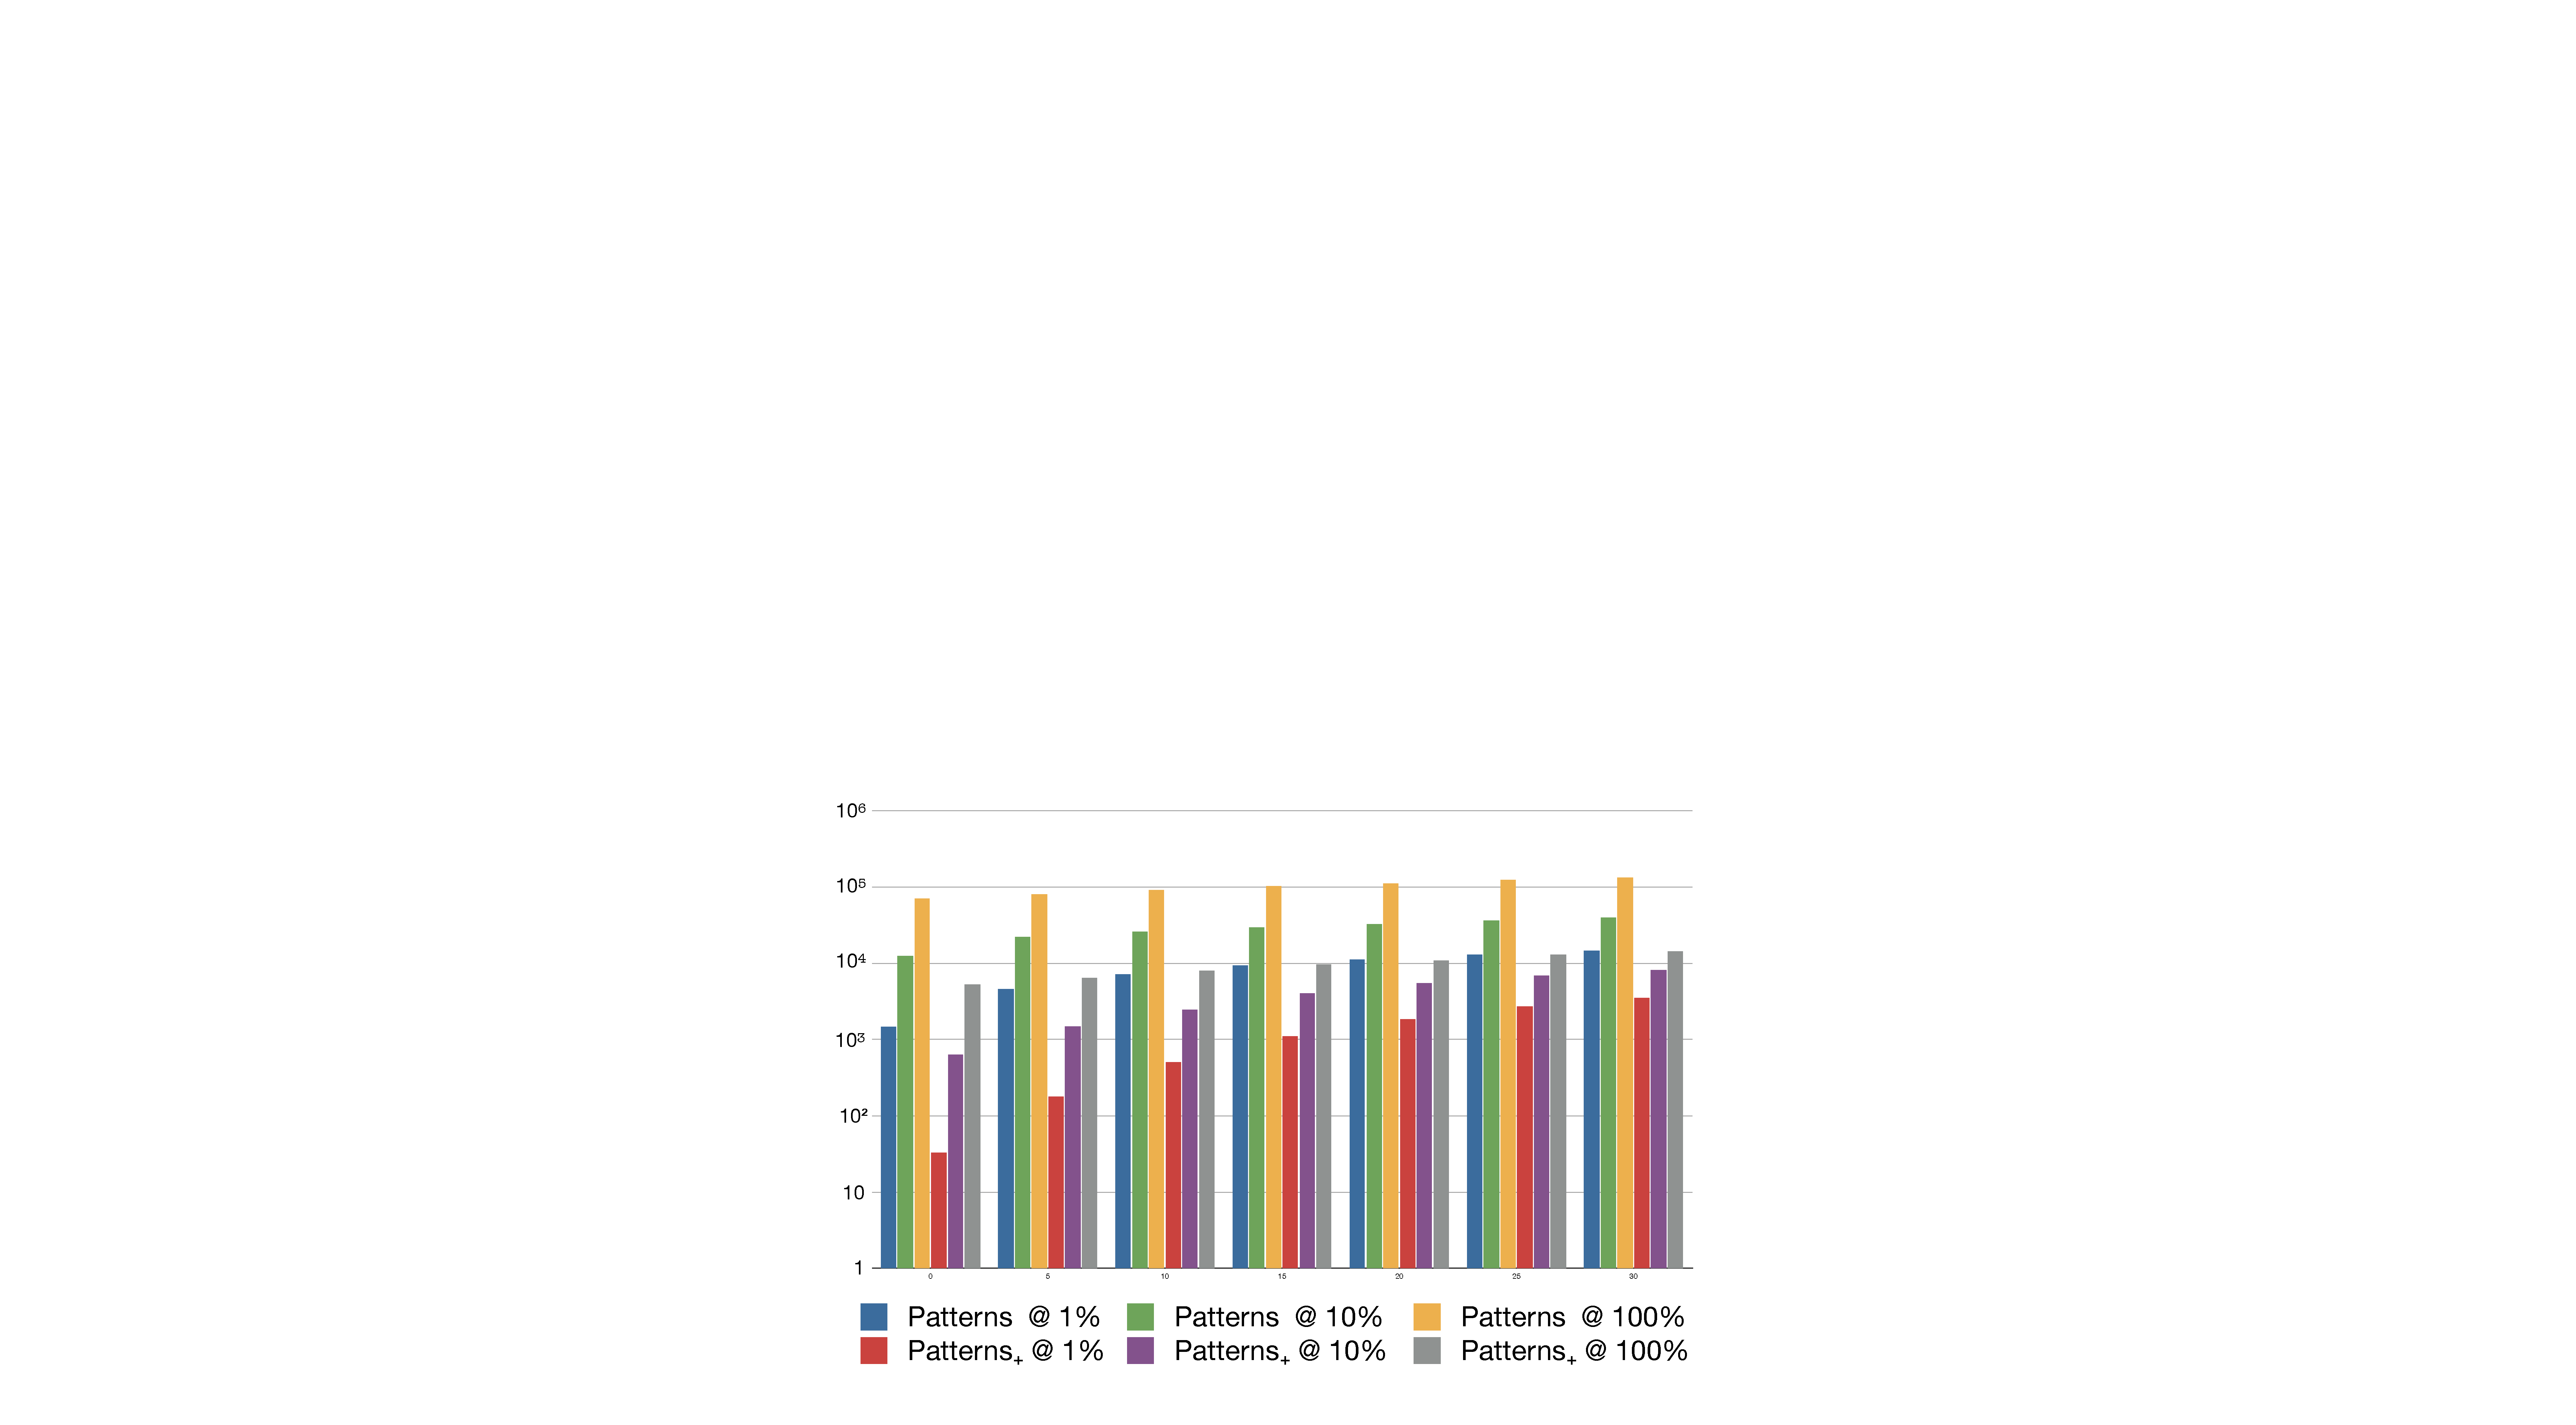
\includegraphics[width=\columnwidth]{images/patterns.pdf}
  \caption{Number of patterns (log scale) and patterns with $|\mathcal{S}_\theta'| > 1$ ($\text{Patterns}_+$) for iterations and test corpus.}
	\label{fig:patterns}
\end{minipage}%
\hspace{0.02em}
\begin{minipage}{.49\textwidth}
  \centering
    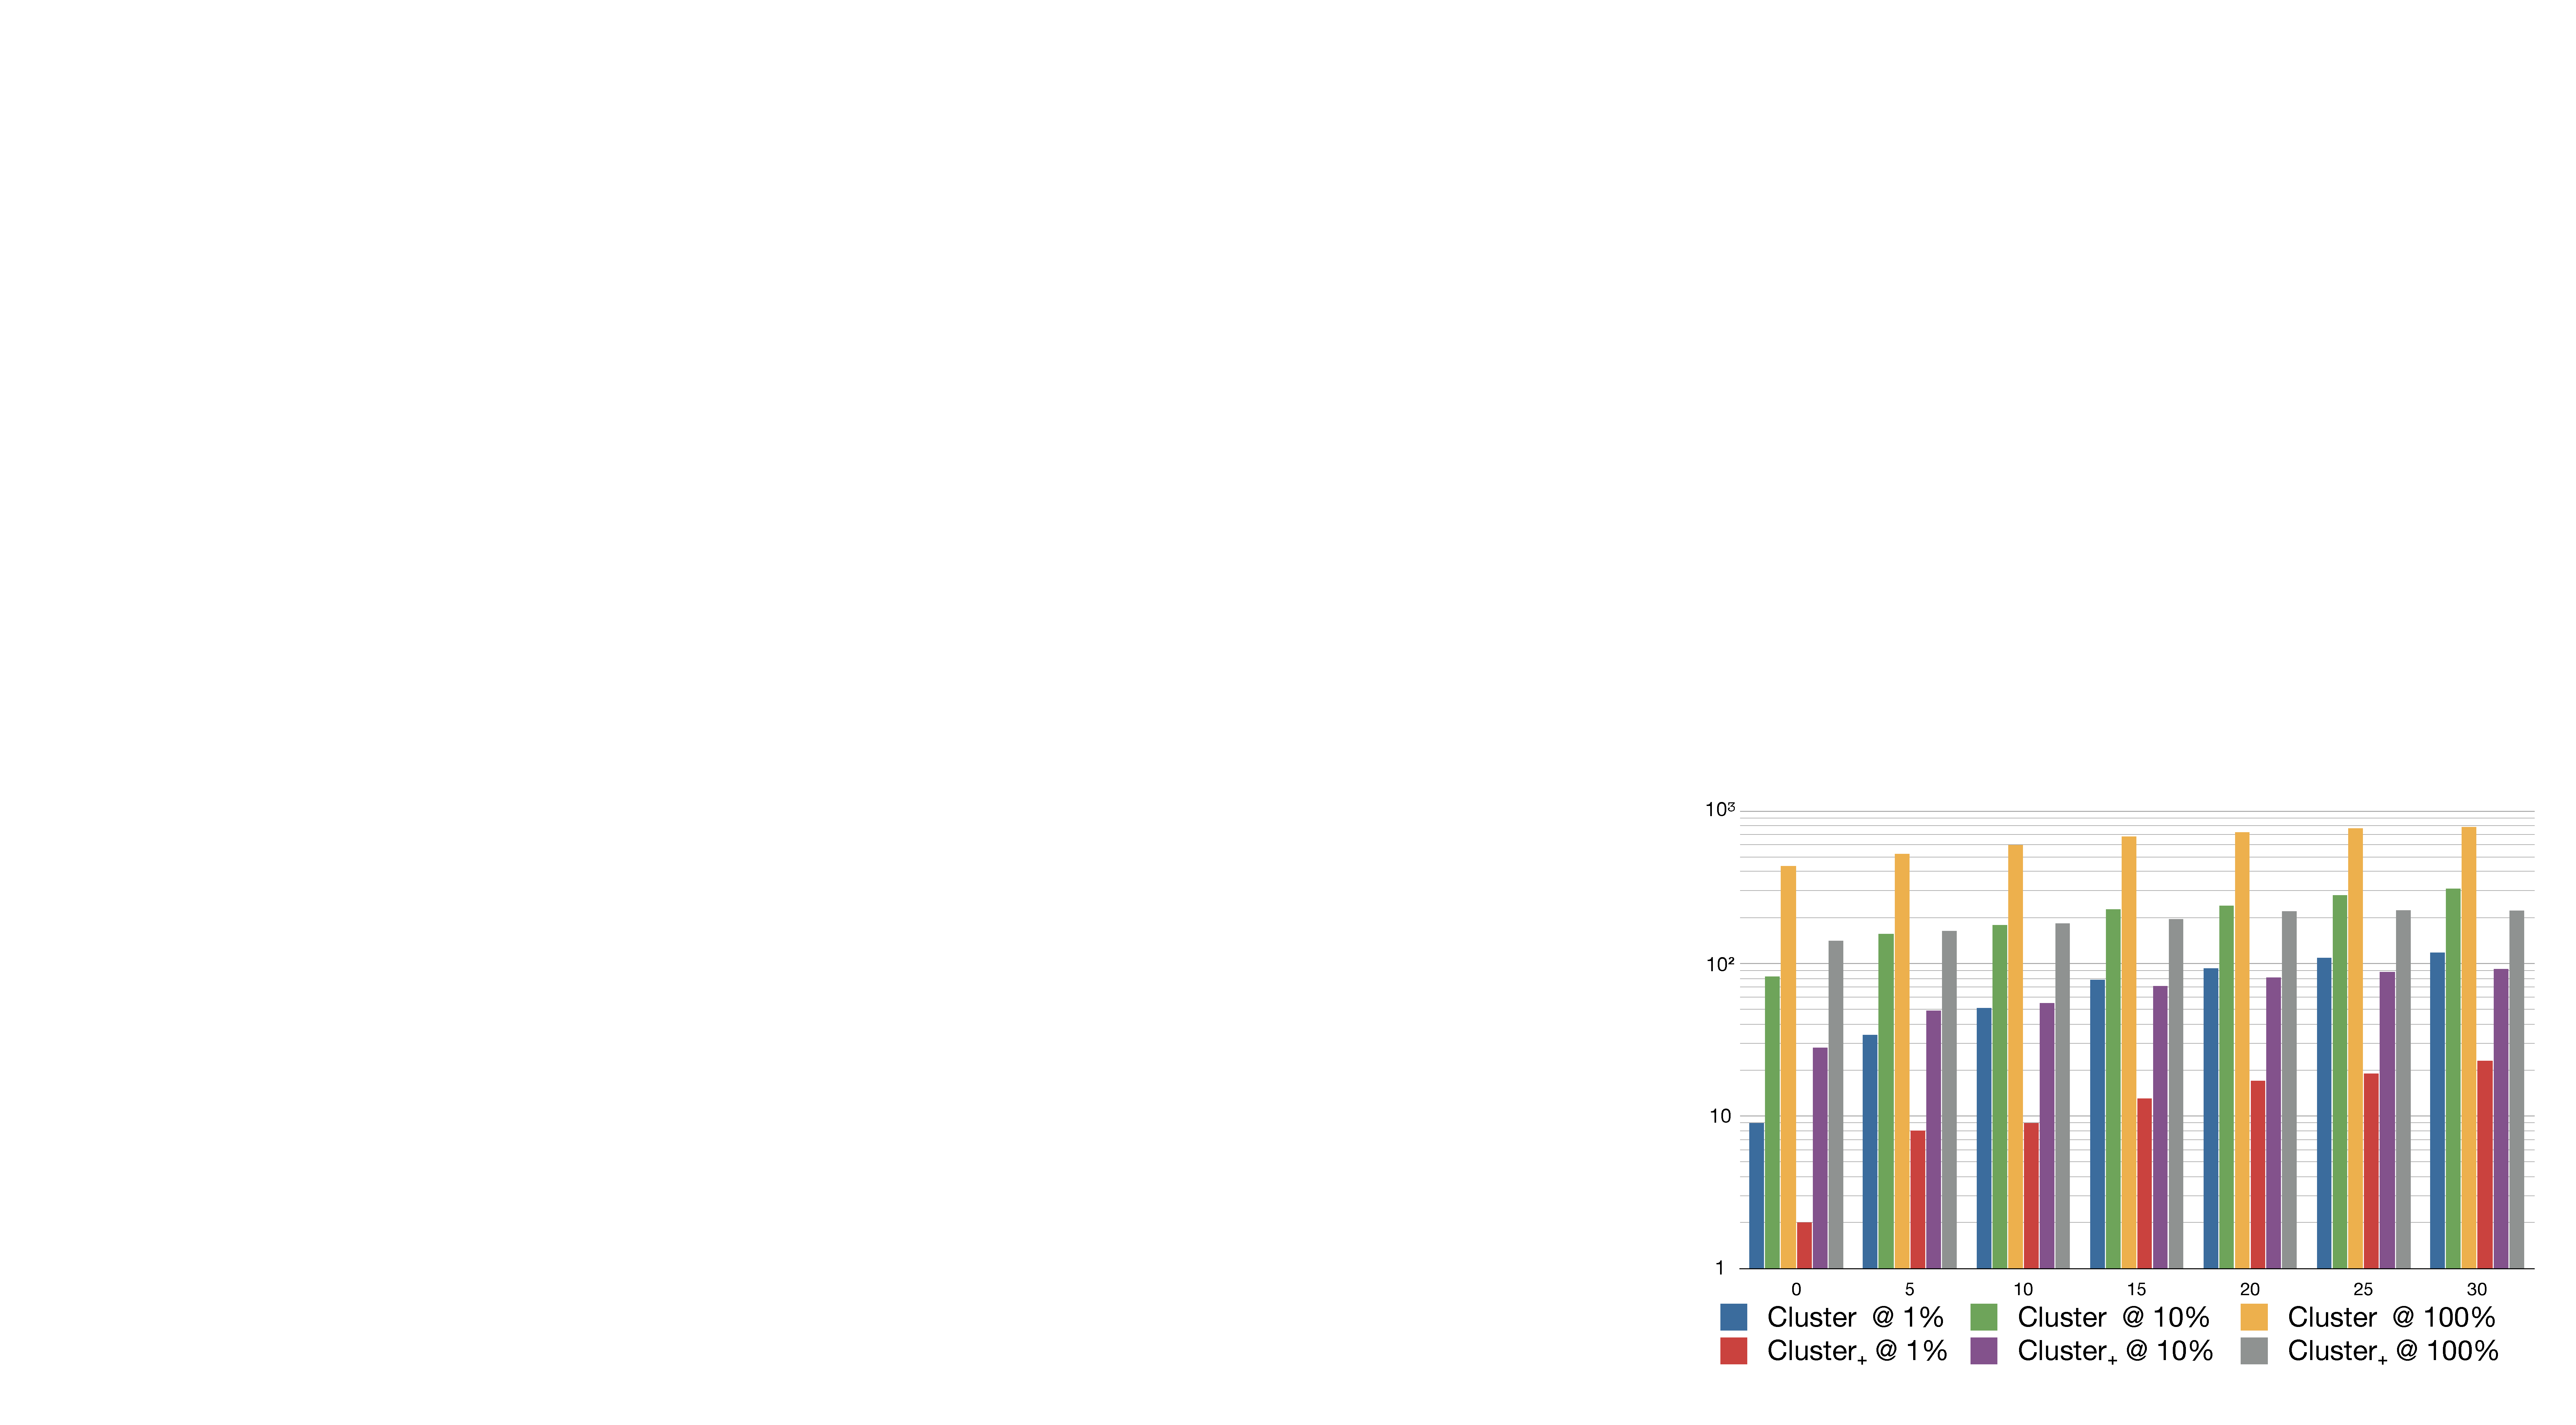
\includegraphics[width=0.97\columnwidth]{images/clusters.pdf}
  \caption{Number of clusters (log scale) and clusters with $|\mathcal{C}| > 1$ ($\text{Cluster}_+$) for iterations and test corpus.}
	\label{fig:clusters}
\end{minipage}
\end{figure}

The results of the growth evaluation for clusters can be seen in Figure~\ref{fig:clusters}.
The evaluation shows that the number of clusters increases by a factor of 2.5 from 1\% to 10\% and 10\% to 100\%.
Moreover, approximately 25\% of all cluster have more than 1 pattern and the number of clusters grows linear for 1\% and 10\% but for the 100\% corpus it seems to coverage to 800.
The same holds true for clusters with more then one pattern, as they stop to grow at around 225 clusters.
%, which would indicate that the number of distinct relations is limited

\section{Related Work}
\label{sec:related_work}
While Semantic Web applications rely on formal, machine understandable languages such as RDF and OWL, enabling powerful features such as reasoning and expressive querying, humans use Natural Language (NL) to express semantics.
This gap between the two different languages has been filled by Information Extraction (IE) approaches, developed by the Natural Language Processing (NLP) research community \cite{Sarawagi:2008:IE:1498844.1498845}, whose goal is to find desired pieces of information, such as concepts (hierarchy of terms which are used to point to shared definitions), entities (name, numeric expression, date) and facts in natural language texts and print them in a form that is suitable for automatic querying and processing.
Ever since the advent of the Linked Open Data initiative\footnote{\url{http://linkeddata.org/}}, IE is also an important key enabler for the Semantic Web.
%, resulting into an increasing demand for the extraction of RDF from unstructured data, as in 
For example, LODifier~(\cite{lodifier}, \cite{entity_extraction}) combines deep semantic analysis with named entity recognition, word-sense disambiguation and controlled Semantic Web vocabularies.
FOX~\cite{DBLP:conf/semweb/NgomoHLSK11} uses ensemble learning to improve the F-score of IE tools.
 %, in which the problem with the diverse strengths and weaknesses of several NLP tools is tackled by combining them and aggregating the results by using neural networks.
The BOA framework~\cite{Gerber2011} uses structured data as background knowledge for the extraction of natural language patterns, which are subsequently employed to extract additional RDF data from natural language text. %, which is finally fed back into the Data Web.%, therewith closing the loop.
%Compared to the batch-oriented IE of static content and driven by the increasing amount of dynamic content (e.g. news, feeds and blogs), t
The authors of~\cite{Nakashole:2012:RPK:2391200.2391208} propose a simple model for fact extraction in real-time taking into account the difficult challenges that timely fact extraction on frequently updated data entails.
A specific application for the news domain is described in~\cite{Stern:2012:PKB:2391200.2391207}, wherein a knowledge base of entities for the French news agency AFP is populated.

%Systems which do not require a pre-specified vocabulary are referred as Open IE systems.
State-of-the-art open-IE systems such as ReVerb automatically identify and extract relationships from text, relying on (in the case of ReVerb) simple syntactic constraints expressed by verbs~\cite{conf/emnlp/FaderSE11}.
The authors of~\cite{conf/acl/DavidovR08} present a novel pattern clusters method for nominal relationship classification using an unsupervised learning environment, which makes the system domain and language-independent.
\cite{Ruiz-Casado:2007:ALL:1238147.1238395} shows how lexical patterns and semantic relationships can be learned from concepts in Wikipedia.

\section{Conclusion and Future Work}

In this paper, we presented \NAME{}, a framework for the extraction of RDF from unstructured data streams.
We presented the components of the \NAME{} framework and evaluated its disambiguation, clustering, linking and scalability capabilities as well as its extraction quality.
We are able to disambiguate resources with a precision of 85\%, cluster patterns with an accuracy of 82.5\% and extract RDF with an total accuracy of around 90\% and handle two hour time slices with around 300.000 sentences within 20 min on a small server.
%\todo{was vielleciht etwas seltsam klingen mag ist, das die einzelschritte weniger precision haben als die total accurracy, liegt daran das die total acc ja nur für cluster sizes gt 4 gilt und die anderen evals sowas nicht berücksichtigen}
In future work, we will extend our approach to also cover datatype properties.
For example from the sentence ``\dots, Google said Motorola Mobility contributed revenue of US\$ 1.25 billion for the second quarter.'' the triple \textit{dbpedia:Google rlno:says ``Motorola Mobility contributed revenue of US\$ 1.25 billion for the second quarter''} can be extracted.
Additionally we plan to integrate DeFacto~\cite{LEH+12a}, which is able to verify or falsify a triple extracted by \NAME{}.
Finally, we will extend our approach with temporal logics to explicate the temporal scope of the triples included in our knowledge base.
%
% The following two commands are all you need in the
% initial runs of your .tex file to
% produce the bibliography for the citations in your paper.

\bibliographystyle{abbrv}
\bibliography{rdflivenews}
% sigproc.bib is the name of the Bibliography in this case
% You must have a proper ".bib" file
%  and remember to run:
% latex bibtex latex latex
% to resolve all references
%
% ACM needs 'a single self-contained file'!
%
%APPENDICES are optional
%\balancecolumns

\end{document}

    